\section{Code Readability}\label{section:code}
Orthogonal to the correctness, readability is another important quality of a piece of code: though not related to the execution results of the code, code readability may significantly affect the usability, upgradability, and ease of maintenance of an entire codebase. 
In this section, we consider the problem of improving the readability of code with \ours. 
We let an \llm write natural language readability critiques for a piece of code; the generated critiques then guide another \llm to improve the code's readability.

\subsection{Method}
Following the \ours setup, we instantiate \initmod, \fbmod, and \itermod.
The \initmod is a no-op --- we directly start by critiquing the code with \fbmod and applying the changes with \itermod.
\begin{itemize}
\item \textbf{\fbmod} We prompt an \llm with the given code and an instruction to provide feedback on readability.
We give the \llm the freedom to freely choose the type of enhancements and express them in the form of free text.
\item \textbf{\itermod} The code generator \llm is prompted with the piece of code and the readability improvement feedback provided by \fbmod. In addition, we also supply an instruction to fix the code using the feedback. We take the generation from the code generator as the product of one iteration in the feedback loop.
\end{itemize}
Starting from an initial piece of code $y_0$, we first critique, $c_1 = \text{critique}(y_0)$, and then edit the code, $y_1 = \text{editor}(y_0, c_1)$. This is recursively performed $N$ times, where $c_{k+1} = \text{critique}(y_k)$ and $y_{k+1} = \text{editor}(y_k, c_{k+1})$.
\subsection{Experiments}
\paragraph{Dataset} We use the CodeNet~\cite{puri2021codenet} dataset of competitive programming.\footnote{\url{https://github.com/IBM/Project_CodeNet}}
For our purpose, these are hard-to-read multi-line code snippets. We consider a random subset of 300 examples and apply \ours to them.

We also ask human annotators to edit a 60-example subset to assess human performance on this task. The human annotators are asked to read the code piece and improve its readability. 

\paragraph{Implementation} Both the critique and the editor models are based on the InstructGPT model~(text-davinci-003). We consider the temperature of both $T=0.0$~(greedy) and $T=0.7$~(sampling) for decoding \emph{Natural Language} suggestion from the critique model. We always use a temperature $T=0.0$~(greedy) when decoding \emph{Programming Language} from the code editor. Due to budget constraints, we run \ours for  $N=5$ iterations. The exact prompts we use can be found in Figures \ref{fig:prompt:readability:fb}-\ref{fig:prompt:readability:refine}.

\paragraph{Evaluation Methods}
We consider a few automatic heuristic-based evaluation metrics,
\begin{itemize}
    \item Meaningful Variable Names: In order to understand the flow of a program, having semantically meaningful variable names can offer much useful information. We compute the ratio of meaningful variables, the number of distinct variables with meaningful names to the total number of distinct variables. We automate the process of extracting distinct variables and the meaningful subset of variables using a few-shot prompted language model.
    \item Comments: Natural language comments give explicit hints on the intent of the code. We compute the average number of comment pieces per code line.
    \item Function Units: Long functions are hard to parse. Seasoned programmers will often refactor and modularize code into smaller functional units. 
\end{itemize}

\paragraph{Result}
For each automatic evaluation metric, the ratio of meaningful variable, of comment, and the number of function units, we compute for each iteration averaged across all test examples and plot for each \ours iteration in \autoref{fig:read:var}, \autoref{fig:read:comment} and \autoref{fig:read:func} respectively. The two curves each correspond to critique with temperature $T=0.0$ and $T=0.7$. The iteration 0 number is measured from the original input code piece from CodeNet. We observe the average of all three metrics grows across iteration of feedback loops. A diverse generation of a higher temperature in the critique leads to more edits to improve the meaningfulness of variable names and to add comments. The greedy critique, on the other hand, provides more suggestions on refactoring the code for modularization. \autoref{fig:code:code-iterations} provides an example of code-readability improving over iterations. 

In \autoref{tab:code-human}, we measure human performance on all three metrics and compare with \ours last iteration output. At $T=0.7$, \ours produces more meaning variables, more function units and slightly more comments compared to the human annotators on average. At $T=0.0$,  \ours produces less meaningful variables, less comments per line but even more function units. 

\begin{table}[]
\centering
\begin{tabular}{c | c | c | c}
  \hline
   & Meaningful Variable Ratio  & Comment Per Line  & Function Units \\
  \hline
  Human Annotator Rewrites & 0.653 & 0.24 & 0.70 \\
  \ours  (T = 0.0)  & 0.628 & 0.12 & \textbf{1.41} \\
  \ours  (T = 0.7)  & \textbf{0.700} & \textbf{0.25} & 1.33 \\
  \hline
\end{tabular}
\caption{Human v.s. \ours performance on 60-example subset. We see \ours can reach similar or achieve even better performance on the metrics compared to rewrites given by human annotator.}
\label{tab:code-human}
\end{table}

\begin{figure}[h]
\centering
\begin{subfigure}[t]{0.32\textwidth}
\begin{adjustbox}{width=\textwidth}
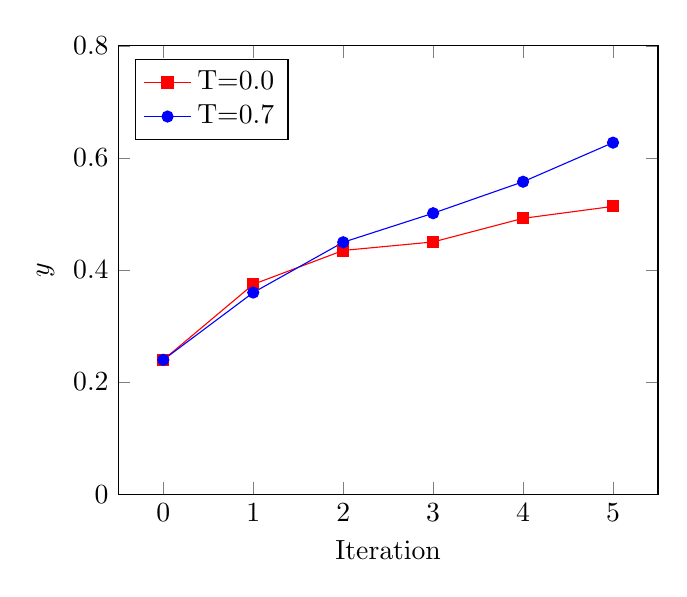
\begin{tikzpicture}
  \begin{axis}[
    xlabel={Iteration},
    ylabel={$y$},
    ymin=0, ymax=0.8,
    xtick={0,1,2,3,4,5},
    ytick={0,0.2,0.4,0.6,0.8},
    legend pos=north west,
    ]
    \addplot[color=red,mark=square*] coordinates {
      (0,0.23963550550903984)
      (1,0.3743883746776086)
      (2,0.43483512163096444)
      (3,0.4500028560477478)
      (4,0.4921556556936677)
      (5,0.5134542852630356)
    };
    \addplot[color=blue,mark=*] coordinates {
      (0,0.23963550550903984)
      (1,0.3597037206410946)
      (2,0.44946686126742497)
      (3,0.5012589804411456)
      (4,0.557436438464786)
      (5,0.6272203279260107)
    };
    
    \legend{T=0.0, T=0.7}
  \end{axis}
\end{tikzpicture}
\end{adjustbox}
\caption{Meaningful variable ratio across different \ours iterations.}
\label{fig:read:var}
\end{subfigure}
~
\begin{subfigure}[t]{0.32\textwidth}
\begin{adjustbox}{width=\textwidth}
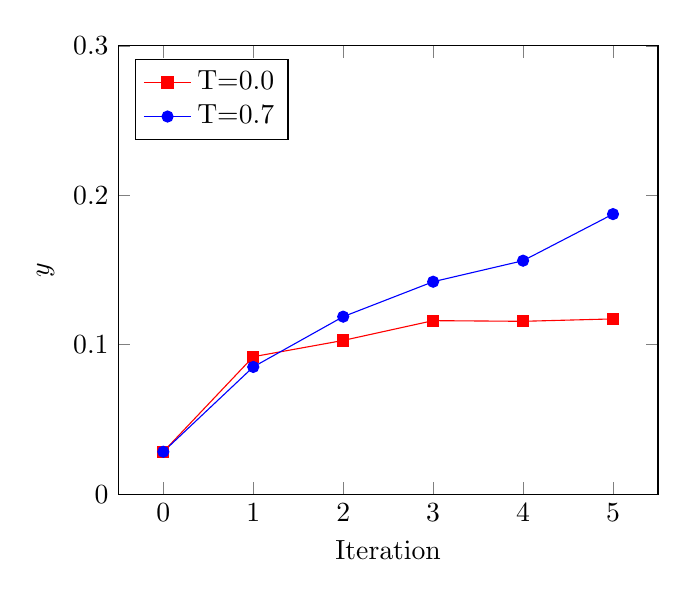
\begin{tikzpicture}
  \begin{axis}[
    xlabel={Iteration},
    ylabel={$y$},
    ymin=0, ymax=0.3,
    xtick={0,1,2,3,4,5},
    ytick={0,0.1, 0.2,0.3},
    legend pos=north west,
    ]
    \addplot[color=red,mark=square*] coordinates {
      (0,0.028369348895543454)
      (1,0.09194571888720554)
      (2,0.10284188610613403)
      (3,0.11608742839681675)
      (4,0.11564706008229259)
      (5,0.11724822210242714)
    };
    \addplot[color=blue,mark=*] coordinates {
      (0,0.028369348895543454)
      (1,0.08511136094717932)
      (2,0.11875152052882809)
      (3,0.14213049815399667)
      (4,0.15619882931403242)
      (5,0.18738499703144273)
    };
    
    \legend{T=0.0, T=0.7}
  \end{axis}
\end{tikzpicture}
\end{adjustbox}
\caption{Comment per line ratio across different \ours iterations.}
\label{fig:read:comment}
\end{subfigure}
~
\begin{subfigure}[t]{0.32\textwidth}
\begin{adjustbox}{width=\textwidth}
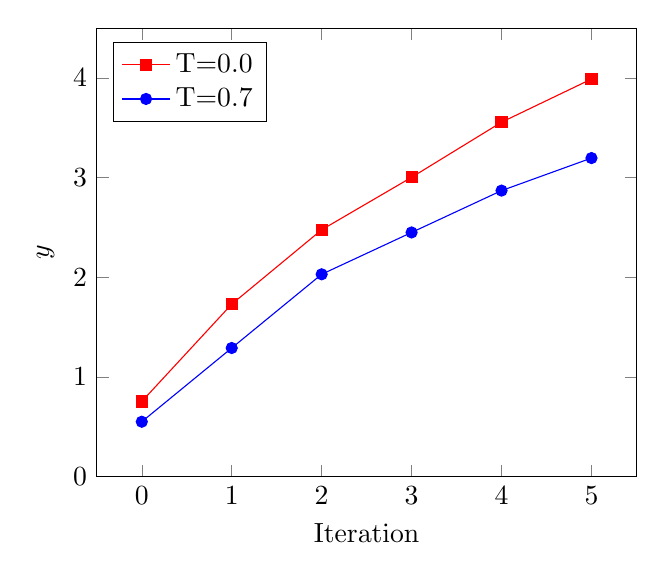
\begin{tikzpicture}
  \begin{axis}[
    xlabel={Iteration},
    ylabel={$y$},
    ymin=0, ymax=4.5,
    xtick={0,1,2,3,4,5},
    ytick={0, 1, 2, 3, 4},
    legend pos=north west,
    ]
    \addplot[color=red,mark=square*] coordinates {
      (0,0.7533333333333333)
      (1,1.73)
      (2,2.4766666666666666)
      (3,3.0033333333333334)
      (4,3.5566666666666666)
      (5,3.99)
    };
    \addplot[color=blue,mark=*] coordinates {
      (0,0.55)
      (1,1.29)
      (2,2.03)
      (3,2.45)
      (4,2.87)
      (5,3.1966666666666668)
    };
    
    \legend{T=0.0, T=0.7}
  \end{axis}
\end{tikzpicture}
\end{adjustbox}
\caption{Number of function units across different \ours iterations.}
\label{fig:read:func}
\end{subfigure}
\caption{Evaluation on code readability task with \ours across multiple metrics}
\end{figure}

\paragraph{Example}

\begin{figure*}[t!]
\textbf{Starting Code: $v_0$} 
\begin{minted}[fontsize=\footnotesize, frame=single]{python}
print((int((int(eval(input()))+1)/2)))
\end{minted}

\textbf{Code $v_1$}
\begin{minted}[fontsize=\footnotesize, breaklines, frame=single]{python}
print(
    (int(
        (int(eval(input())) + 1)
        / 2
    )
)
\end{minted}

    
\textbf{Code $v_2$}
\begin{minted}[fontsize=\footnotesize, breaklines, frame=single]{python}
num_input = eval(input())
num_input = int(num_input)
num_input += 1
num_result = int(num_input / 2)
print(num_result)
\end{minted}

\caption{\ours iterations over a piece of densely composed code. Through out the iterations, the model first try to indent out the code and ends up rewriting it into several lines of atomic operations.
}
\label{fig:code:code-iterations}
\end{figure*}